\section{Arquitetura}

\subsection{Representação da Arqitetura}

A forma como o \textit{framework} Ionic está sendo utilizado pode ser representada por um diagrama de pacotes (Figura \ref{img:pacotes}):

\begin{figure}[H]
    \centering
    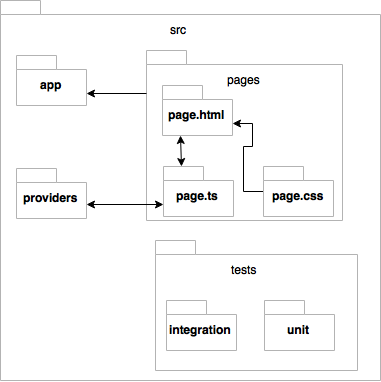
\includegraphics[scale=0.5]{figuras/ionic_arch.png}
    \caption[Diagrama de pacotes do aplicativo]{Diagrama de pacotes. Fonte: autores}
    \label{img:pacotes}
\end{figure}
\pagebreak

\begin{itemize}
\item\textbf{\textit{src}}: é o diretório fonte da aplicação, onde os principais recursos serão salvos.
\item\textbf{\textit{app}}: onde o \textit{framework} reúne todos os recursos a serem compilados.
\item\textbf{\textit{pages}}: as páginas do aplicativo, como o login, a página de registro de contas, entre outras. Cada página é composta de HTML e CSS, que compõem o visual da página e o Typescript que é onde está a parte lógica;
\item\textbf{\textit{providers}}: os métodos que fazem a comunicação da API com o aplicativo.
\item\textbf{\textit{tests}}: os diferentes tipos de testes de software realizados no applicativo.
\item\textbf{\textit{integration}}: testes de integração.
\item\textbf{\textit{unit}}: testes de unidade.
\end{itemize}

A arquitetura da API é baseada na arquitetura MVC e foi definida como ilustra a Figura \ref{img:arquitetura}:

\begin{figure}[H]
    \centering
    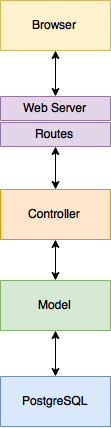
\includegraphics[scale=0.5]{figuras/api_arch.png}
    \caption[Arquitetura da API]{Arquitetura da API. Fonte: autores}
    \label{img:arquitetura}
\end{figure}

As classes modelos se comunicam com o banco de dados \textit{PostgreSQL} e com as classes controladoras, que por sua vez enviam e recebem dados para as rotas que são disponibilizadas por um servidor web; o usuário pode acessar esses dados via navegador ou outro tipo de aplicação cliente.

\subsection{Modelo de Dados}

Utilizando a ferramenta MySQL Workbench, foi criado um modelo de dados da aplicação. O dicionário de dados pode ser encontrado no Apêndice \ref{chap:dicionario}. O modelo da aplicação é representado pela Figura \ref{img:modelo_de_dados}.

\begin{figure}[H]
    \centering
    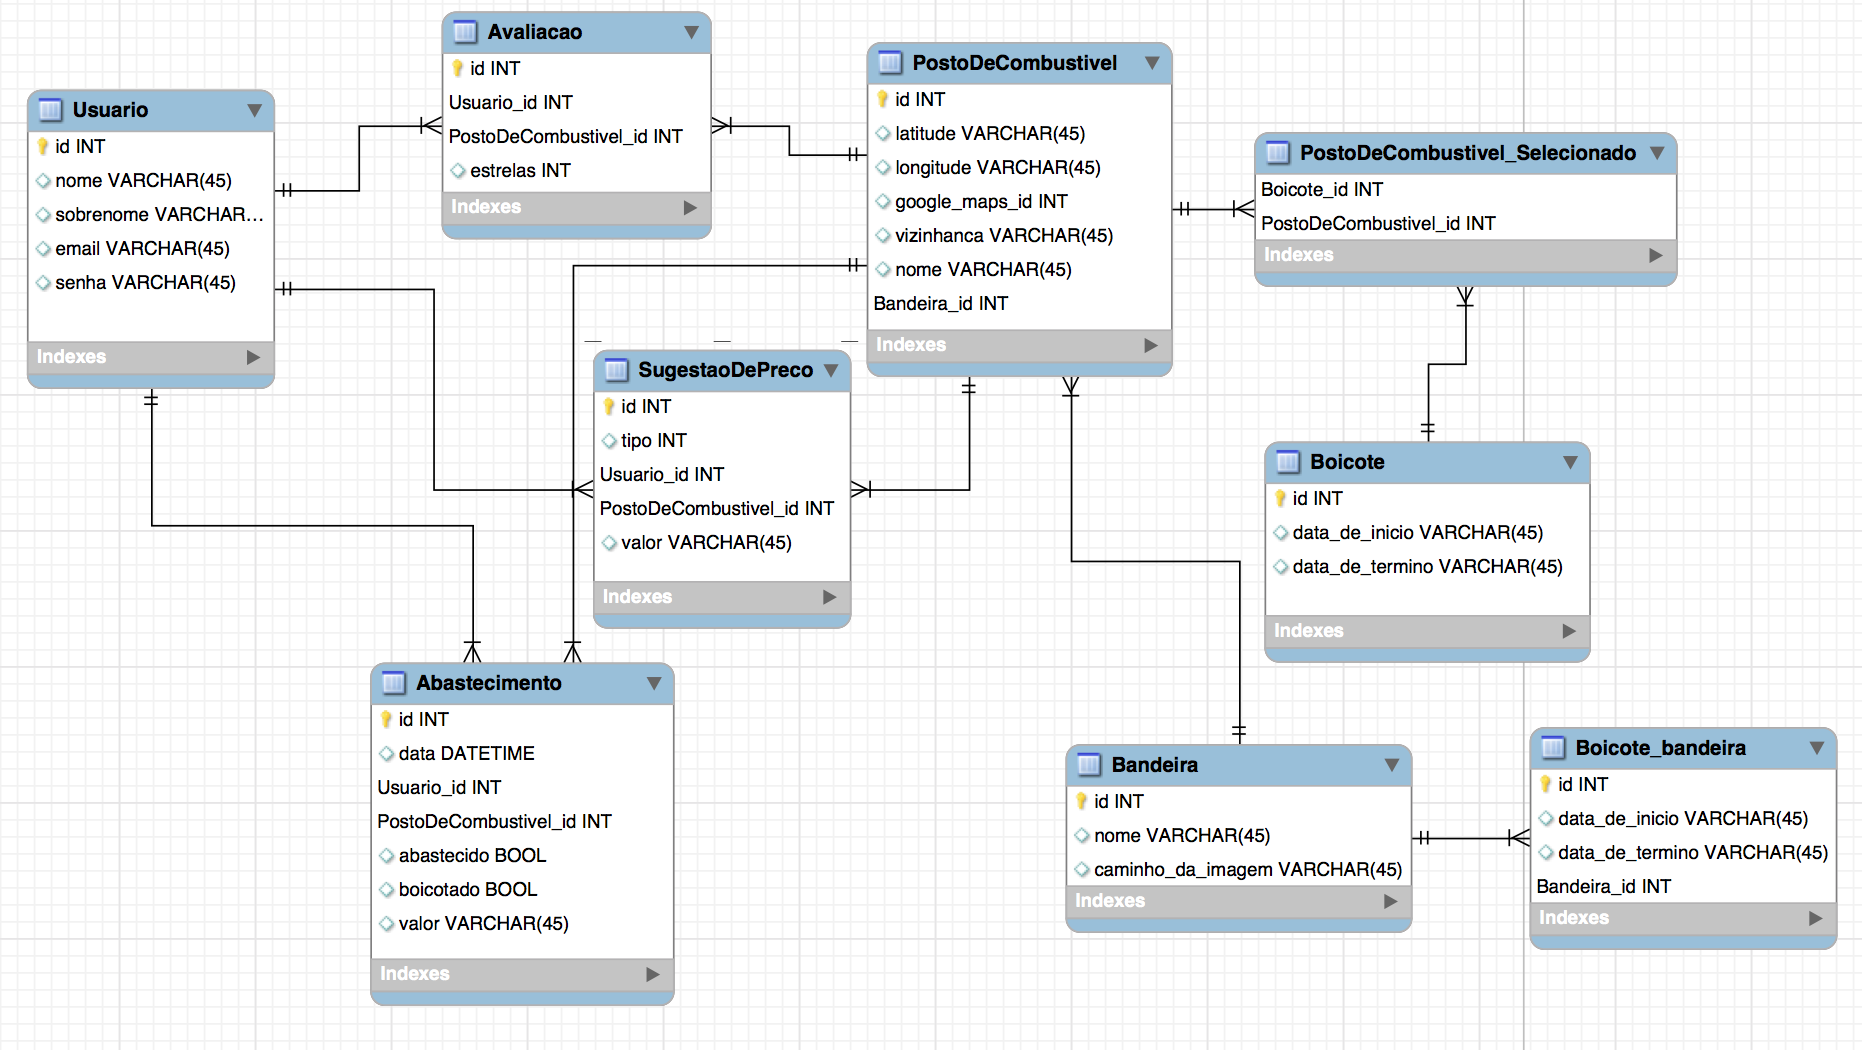
\includegraphics[scale=0.5]{figuras/modelagem_traduzida.png}
    \caption[Modelo de dados]{Modelo de dados Fonte: autores}
    \label{img:modelo_de_dados}
\end{figure}
